\subsection{Integration theory}

DEFINITION 13. --- Let \(p \in [1, +\infty[\) ; one denotes by \(\overline{\mathcal{L}}^p(T, \mu)\) (resp. \(\overline{\mathcal{L}}_F^p(T, \mu)\) if \(F\) is a Banach space) the set of mappings \(f\) of \(T\) into \(\overline{R}\) (resp. into \(F\) ) that are \(\mu\) -measurable and satisfy \(\mu^\bullet(|f|^p) < +\infty\) . One denotes by \(\mathcal{L}^p(T, \mu)\) (resp. \(\mathcal{L}_F^p(T, \mu)\) ) the set of \(\mu\) -moderated elements of \(\overline{\mathcal{L}}^p(T, \mu)\) (resp. \(\overline{\mathcal{L}}_F^p(T, \mu)\) ).

We will write \(\overline{\mathbf{N}}_p(\mathbf{f}) = (\mu^\bullet (|\mathbf{f}|^p))^{1 / p}\) , \(\mathrm{N}_p(\mathbf{f}) = (\mu^* (|\mathbf{f}|^p))^{1 / p}\) . We denote by \(\overline{\mathrm{N}}_{\infty}(\mathbf{f})\) the infimum of the numbers \(k\geqslant 0\) such that \(|\mathbf{f}|\leqslant k\) locally \(\mu\) -almost everywhere; if \(\overline{\mathrm{N}}_{\infty}(\mathbf{f}) < + \infty\) , \(\mathbf{f}\) is said to be essentially bounded. The set of measurable and essentially bounded mappings of T into \(\overline{\mathbf{R}}\) (resp. into F) is denoted \(\overline{\mathcal{L}}^{\infty}(\mathrm{T},\mu)\) (resp. \(\overline{\mathcal{L}}_{\mathrm{F}}^{\infty}(\mathrm{T},\mu)\) ). The elements of \(\overline{\mathcal{L}}_{\mathrm{F}}^{1}(\mathrm{T},\mu)\) (resp. \(\mathcal{L}_{\mathrm{F}}^{1}(\mathrm{T},\mu)\) ) are called essentially integrable functions (resp. integrable functions) with values in F.

If \(\mu\) is a complex measure, one sets

\[
\overline {{{{\mathcal {L}}}}} _ {\mathrm{F}} ^ {p} (\mathrm{T}, \mu) = \overline {{{{\mathcal {L}}}}} _ {\mathrm{F}} ^ {p} (\mathrm{T}, | \mu |) \quad \text { and } \quad \mathcal {L} _ {\mathrm{F}} ^ {p} (\mathrm{T}, \mu) = \mathcal {L} _ {\mathrm{F}} ^ {p} (\mathrm{T}, | \mu |).
\]

The above notations are often abbreviated to \(\overline{\mathcal{L}}_F^p (\mu)\) , \(\overline{\mathcal{L}}_F^p\) or \(\mathcal{L}^p (\mu)\) , \(\mathcal{L}^p\) , if this does not lead to any confusion.

We saw in No.~8 (Scholium) that one can construct a locally compact space \(\mathbf{T}'\) , having the same underlying set as \(\mathbf{T}\) and a topology finer than that of \(\mathbf{T}\) , and equip \(\mathbf{T}'\) with a measure \(\mu'\) such that the \(\mu\) -measurable functions and the \(\mu'\) -measurable functions are the same, and such that the essential upper integrals of positive functions for \(\mu\) and \(\mu'\) are equal. It follows that the sets \(\overline{\mathcal{L}}_{\mathrm{F}}^{p}(\mu)\) and \(\overline{\mathcal{L}}_{\mathrm{F}}^{p}(\mu')\) are identical for \(1 \leqslant p \leqslant +\infty\) . (1) This also implies without new proof that \(\overline{\mathcal{L}}_{\mathrm{F}}^{p}\) is a vector space, and that the function \(\overline{\mathrm{N}}_p\) is a semi-norm on \(\overline{\mathcal{L}}_{\mathrm{F}}^{p}(\mu)\) , for which this space is complete.

Let \(\mathbf{f}\) be an element of \(\overline{\mathcal{L}}_{\mathrm{F}}^{p}\) ( \(1 \leqslant p < +\infty\) ); since one has \(\mu^{\bullet}(|\mathbf{f}|^{p}) = \mu^{\prime \bullet}(|\mathbf{f}|^{p}) < +\infty\) , Prop. 7 of Ch. V, §1, No.~2 implies that \(\mathbf{f}\) is zero outside the union of a sequence of compact subsets of \(\mathbf{T}'\) and a locally \(\mu'\) -negligible set; the latter set being locally \(\mu\) -negligible, and every compact subset of \(\mathbf{T}'\) being compact in \(\mathbf{T}\) , it follows that \(\mathbf{f}\) is equal locally \(\mu\) -almost everywhere to a \(\mu\) -moderated function. Let us denote by \(\overline{\mathcal{N}}_{\mathrm{F}}\) (resp. \(\mathcal{N}_{\mathrm{F}}\) ) the space of locally \(\mu\) -negligible (resp. \(\mu\) -negligible) functions; we thus have \(\overline{\mathcal{L}}_{\mathrm{F}}^{p} = \mathcal{L}_{\mathrm{F}}^{p} + \overline{\mathcal{N}}_{\mathrm{F}}\) , and \(\mathcal{N}_{\mathrm{F}} = \mathcal{L}_{\mathrm{F}}^{p} \cap \overline{\mathcal{N}}_{\mathrm{F}}\) (No.~9, Cor. 1 of Prop. 14). The space \(\overline{\mathcal{L}}_{\mathrm{F}}^{p} / \overline{\mathcal{N}}_{\mathrm{F}}\) may therefore be canonically identified with \(\mathcal{L}_{\mathrm{F}}^{p} / \mathcal{N}_{\mathrm{F}}\) , and one verifies immediately that this identification preserves norm; this quotient space is denoted \(\mathrm{L}_{\mathrm{F}}^{p}(\mu)\) . It can be interpreted as the normed space associated with each of the semi-normed spaces \(\overline{\mathcal{L}}_{\mathrm{F}}^{p}(\mu)\) and \(\mathcal{L}_{\mathrm{F}}^{p}(\mu)\) ; since \(\overline{\mathcal{L}}_{\mathrm{F}}^{p}\) is complete, the same is true of \(\mathrm{L}_{\mathrm{F}}^{p}\) and \(\mathcal{L}_{\mathrm{F}}^{p}\) .

The set of functions \(\mathbf{f}\) with values in \(\mathbf{F}\) , continuous on \(\mathbf{T}'\) with compact support, is dense in \(\overline{\mathcal{L}}_{\mathbf{F}}^{p}(\mu') = \overline{\mathcal{L}}_{\mathbf{F}}^{p}(\mu)\) (Ch. IV, §3, No.~4, Def. 2). Let us take up again the notations of the Scholium of No.~8. Since a compact subset of \(\mathbf{T}'\) intersects only a finite number of the compact sets \(\mathbf{K}_{\alpha}\) , every continuous function \(\mathbf{f}\) on \(\mathbf{T}'\) with compact support may be written as a sum

\[
\mathbf {f} = \sum_ {\alpha \in A} \mathbf {f} _ {\alpha} + \mathbf {g},
\]

where \(f_{\alpha}\) is, for every \(\alpha\) , the extension by 0 of a continuous function on \(K_{\alpha}\) , where \(f_{\alpha}=0\) except for a finite number of indices, and where g is locally \(\mu\) -negligible. We thus have the following result:

PROPOSITION 15. --- The set of functions f with values in F, such that Supp(f) is compact and such that the restriction of f to Supp(f) is continuous, is dense in \(\overline{\mathcal{L}}_{\mathrm{F}}^{p}(\mu)\) and in \(\mathcal{L}_{\mathrm{F}}^{p}(\mu)\) , for \(1 \leqslant p < +\infty\) .

\pandocbounded{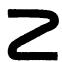
\includegraphics[keepaspectratio]{images/part002_287b28a9.jpg}}

Note that these functions are not continuous functions on T with compact support.

Let us pass to the definition of the integral.

PROPOSITION 16. --- There exists one and only one continuous linear mapping \(\mathbf{f} \mapsto \int \mathbf{f} d\mu\) , of the space \(\overline{\mathcal{L}}_{\mathrm{F}}^{1}(\mu)\) into \(\mathrm{F}\) , having the following property:

If \(\mathbf{f}\) is of the form \(t \mapsto g(t)\mathbf{a}\) , where \(\mathbf{a} \in \mathbf{F}\) , and where \(g\) is a positive function, finite, \(\mu\) -measurable and such that \(\mu^{\bullet}(g) < +\infty\) , then \(\int \mathbf{f} d\mu = \mu^{\bullet}(g) \cdot \mathbf{a}\) .

For, the semi-normed spaces \(\overline{\mathcal{L}}_{\mathrm{F}}^{1}(\mu)\) and \(\overline{\mathcal{L}}_{\mathrm{F}}^{1}(\mu')\) are identical. Since \(\mu^{\bullet} = \mu'^{\bullet}\) , the mapping \(\mathbf{f} \mapsto \int \mathbf{f} d\mu'\) satisfies the conditions of the statement. On the other hand, the set of functions of the form \(\mathbf{f} = g \cdot \mathbf{a}\) considered in the statement is total in \(\overline{\mathcal{L}}_{\mathrm{F}}^{1}(\mu')\) (Ch. IV, §3, No.~5, Prop. 10), whence uniqueness.

One says that \(\int f d\mu\) is the integral of f with respect to \(\mu\) , and this vector is also denoted \(\mu(\mathbf{f})\) or \(\int \mathbf{f}(t) d\mu(t)\) .

Since \(\int f d\mu = \int f d\mu'\) for every essentially integrable function f with values in F, all of the theory of the essential integral extends to measures on Hausdorff spaces, without new proofs; from it, one deduces results relative to the ordinary integral by restricting oneself to moderated functions. We cite in particular the following results:

--- Th. 3 of Ch. IV, §3, No.~4, its extension to \(\overline{\mathcal{L}}_{\mathrm{F}}^{p}\) , and its two corollaries.

--- Th. 4 of Ch. IV, §3, No.~5 (composition with a continuous linear mapping) and its corollaries; Props. 9, 11 and 12 of the same No.

--- All of the results of Ch. IV, §3, No.~6, relative to the ordered vector space structure of \(L^{p}\) .

--- All of the results of Ch. IV, §3, No.~7, and in particular Lebesgue's theorem.

--- All of the results of Ch. IV, §3, No.~8, on the relations between the spaces \(L_F^p\) .

--- Theorem 2 of Ch. IV, §4, No.~3 (the statement of Lebesgue's theorem specific to \(L_F^1\) ).

--- Hölder's inequality (Ch. IV, §6, No.~4, Th. 2) and its corollaries.

--- The relations between the spaces \(L_{F}^{p}\) established in Ch. IV, §6, No.~5.

-- The results on the duality of the spaces \(\mathbf{L}^p\) established in Ch. V, §5, No.~8.

--- The Dunford--Pettis theorem (Ch. VI, §2, No.~5, Th. 1), its Corollaries 1 and 2, and Prop. 10 of Ch. VI, §2, No.~6 (dual of \(L_{F}^{1}\) ).

